\subsection{Tableaux para la lógica de primer orden}
Empezamos con un ejemplo sencillo. Sean 
\[ \varphi_1 \equiv \mbox{ Algunos niños son buenos} \]
\[ \varphi_2 \equiv \mbox{ Todo lo bueno se come} \]
\[ \rule{60mm}{0.1mm} \]
\[ \therefore \mbox{ Algunos niños se comen} \]
para formalizar se ha utilizado 
\[ \mbox{ni}(x) \equiv x \mbox{ es niño} \]
\[ \mbox{co}(x) \equiv x \mbox{ se come} \]
\[ \mbox{bu}(x) \equiv x \mbox{ es bueno} \]

\begin{figure}[h]
\centering
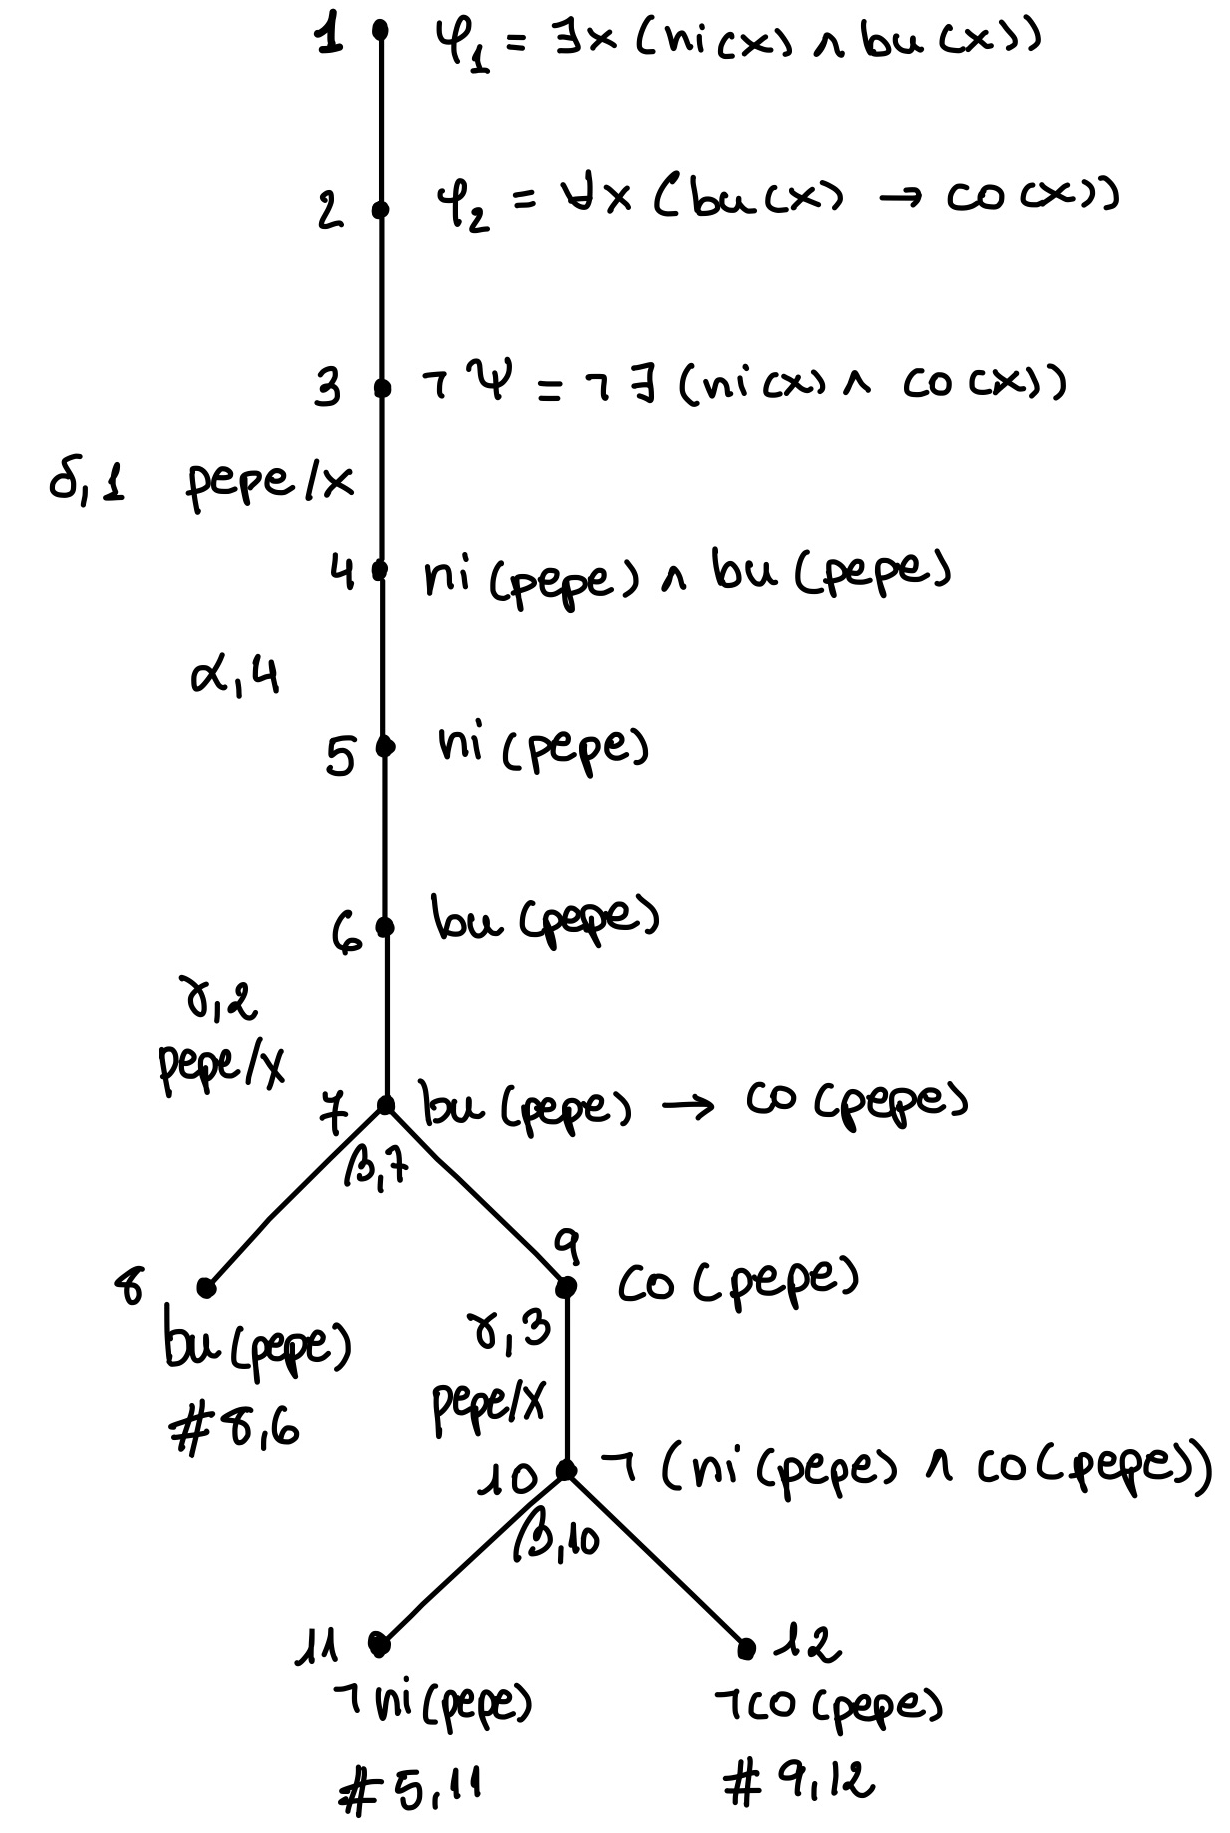
\includegraphics[width=8cm]{arbol_1.png}
\end{figure}

En el ejemplo anterior hemos usado la constante \textit{pepe}. En general supondremos que existe un conjunto de constantes auxiliares 
\[ C_A= \{c_0,  \, c_1, \, c_2, \ldots \} \]
En los tableaux supondremos que estas constantes están siempre en nuestra signatura.  

\subsubsection{Clasificación de fórmulas}
Tomamos de la lógica proposicional las $\alpha$, $\beta$ y $\sigma$ fórmulas. Además, consideramos
\begin{itemize}
	\item $\gamma$-fórmulas, universales 
	\begin{table}[h!]
\centering
\begin{tabular}{c|c}
$\gamma$                   & $\gamma (t)$         \\ \hline
$\forall x \, \varphi$     & $\varphi [t/x]$      \\
$\neg \exists x \, \varphi$ & $\neg \varphi [t/x]$
\end{tabular}
$t \in \term{S}$.
\end{table}
\newpage
	\item $\delta$-fórmulas, existenciales
\begin{table}[h!]
\centering
\begin{tabular}{c|c}
$\delta$                   & $\delta (c)$         \\ \hline
$\neg \forall x \, \varphi$     & $\neg \varphi [c/x]$      \\
$\exists x \, \varphi$ & $\varphi [c/x]$
\end{tabular}
$c \in C_A$
\end{table}
	\item Axiomas de igualdad ($\theta \in \mbox{EQ}_S$) 
	\begin{itemize}
		\item[(RF)] $\forall x \:\: x \doteq x$
		\item[(IM)] $\forall x \forall y \: x \doteq y \rightarrow y \doteq x $
		\item[(IM)] $\forall x \forall y \forall z \: x \doteq y \wedge y \doteq z \rightarrow x \doteq z $
		\item[($\mbox{ST}_1$)] Sustitución para funciones. Si $f\vert_{k} \in \fn{S}$ 
		\[ \forall x_1, \ldots x_k \forall y_1 \ldots, y_k \: x_1 \doteq y_1 \wedge \ldots \wedge x_k \doteq y_k  \rightarrow f(x_1, \ldots x_k) = f( y_1 \ldots, y_k)\]
		\item[($\mbox{ST}_2$)] Sustitución para predicados. Si $p\vert_{k} \in \pd{S}$ 
		\[ \forall x_1, \ldots x_k \forall y_1 \ldots, y_k \: x_1 \doteq y_1 \wedge \ldots \wedge x_k \doteq y_k  \rightarrow p(x_1, \ldots x_k) = p( y_1 \ldots, y_k)\]
	\end{itemize}
\end{itemize}
\subsection{Reglas para la construcción de tableaux}
\begin{itemize}
	\item Las reglas que ya fueron utilizadas en la lógica proposicional aquí son exactamente igual de válidas: $\mbox{R}_{\mbox{ini}}$, $\mbox{R}_{\alpha}$, $\mbox{R}_{\beta}$, $\mbox{R}_\sigma$, $\mbox{R}_{\mbox{hip}}$.
	\item $\mbox{R}_{\gamma}$, si $\gamma$ es fórmula universal y $t \in \term{S}$ un término
	\[\begin{tikzcd}
                      & {} \arrow[d, no head] \arrow[ldd, no head] \arrow[rdd, no head] &    \\
                      & \gamma \arrow[d, no head]                                       &    \\
{} \arrow[r, no head] & {} \arrow[r, no head]                                           & {}
\end{tikzcd} \xrightarrow{\quad \mbox{R}_{\gamma} \quad} \begin{tikzcd}
                      & {} \arrow[d, no head] \arrow[ldd, no head] \arrow[rdd, no head] &    \\
                      & \gamma \arrow[d, no head]                                       &    \\
{} \arrow[r, no head] & {} \arrow[r, no head] \arrow[d, no head]                        & {} \\
                      & \gamma(t)                                                        &   
\end{tikzcd} \]
si $r$ es una rama abierta del árbol y $\gamma \in \Gamma_r$, se puede extender la rama $r$ con $\gamma(t)$.
\item $\mbox{R}_{\delta}$, si $\delta$ es fórmula existencial y $c \in C_A$ una constante 
	\[\begin{tikzcd}
                      & {} \arrow[d, no head] \arrow[ldd, no head] \arrow[rdd, no head] &    \\
                      & \delta \arrow[d, no head]                                       &    \\
{} \arrow[r, no head] & {} \arrow[r, no head]                                           & {}
\end{tikzcd} \xrightarrow{\quad \mbox{R}_{\delta} \quad} \begin{tikzcd}
                      & {} \arrow[d, no head] \arrow[ldd, no head] \arrow[rdd, no head] &    \\
                      & \delta \arrow[d, no head]                                       &    \\
{} \arrow[r, no head] & {} \arrow[r, no head] \arrow[d, no head]                        & {} \\
                      & \delta(t)                                                        &   
\end{tikzcd} \]
si $r$ es una rama abierta del árbol, se puede extender la rama $r$ con $\delta(c)$. Donde $c$ debe ser nueva en la rama.
\item $\mbox{R}_{\theta}$, $\theta \in \mbox{EQ}_S$ 
	\[\begin{tikzcd}
                                           & {} \arrow[d, no head] &                        \\
{} \arrow[ru, no head] \arrow[rr, no head] & {}                    & {} \arrow[lu, no head]
\end{tikzcd} \xrightarrow{\quad \mbox{R}_{\theta} \quad} \begin{tikzcd}
                                           & {} \arrow[d, no head] &                        \\
{} \arrow[ru, no head] \arrow[rr, no head] & {} \arrow[d, no head] & {} \arrow[lu, no head] \\
                                           & \theta               &                       
\end{tikzcd} \]
en cualquier momento se pueden usar los axiomas de igualdad. 
\end{itemize}

Una vez vistas estas reglas, surge de forma natural la cuestión 
\begin{center}
\textit{¿Por qué la constante $c$ debe ser nueva?}
\end{center}
veámoslo a través de un ejemplo.
\paragraph{}
\addtocounter{ej}{1} % sumo 1
\textbf{Ejemplo \arabic{ej}}: 
\[ \begin{matrix}
\mbox{Alguien mató a Trosky}\\
 \mbox{Estalín pagó a Alguien} \\
 \rule{85mm}{0.1mm} \\
 \therefore \mbox{Estalín pagó a alguien que mató a Trosky}
\end{matrix} \qquad \qquad  \begin{matrix}
\exists x \; \mbox{mato}(x, \, \mbox{Trosky}) \\
 \exists x \; \mbox{pago}(\mbox{Stalin}, \, x) \\
 \rule{70mm}{0.1mm} \\
 \therefore \exists x \; \mbox{pago}(\mbox{Stalin}, \, x) \wedge \mbox{mato}(x, \, \mbox{Trosky}) 
\end{matrix}\]


\begin{figure}[h]
\centering
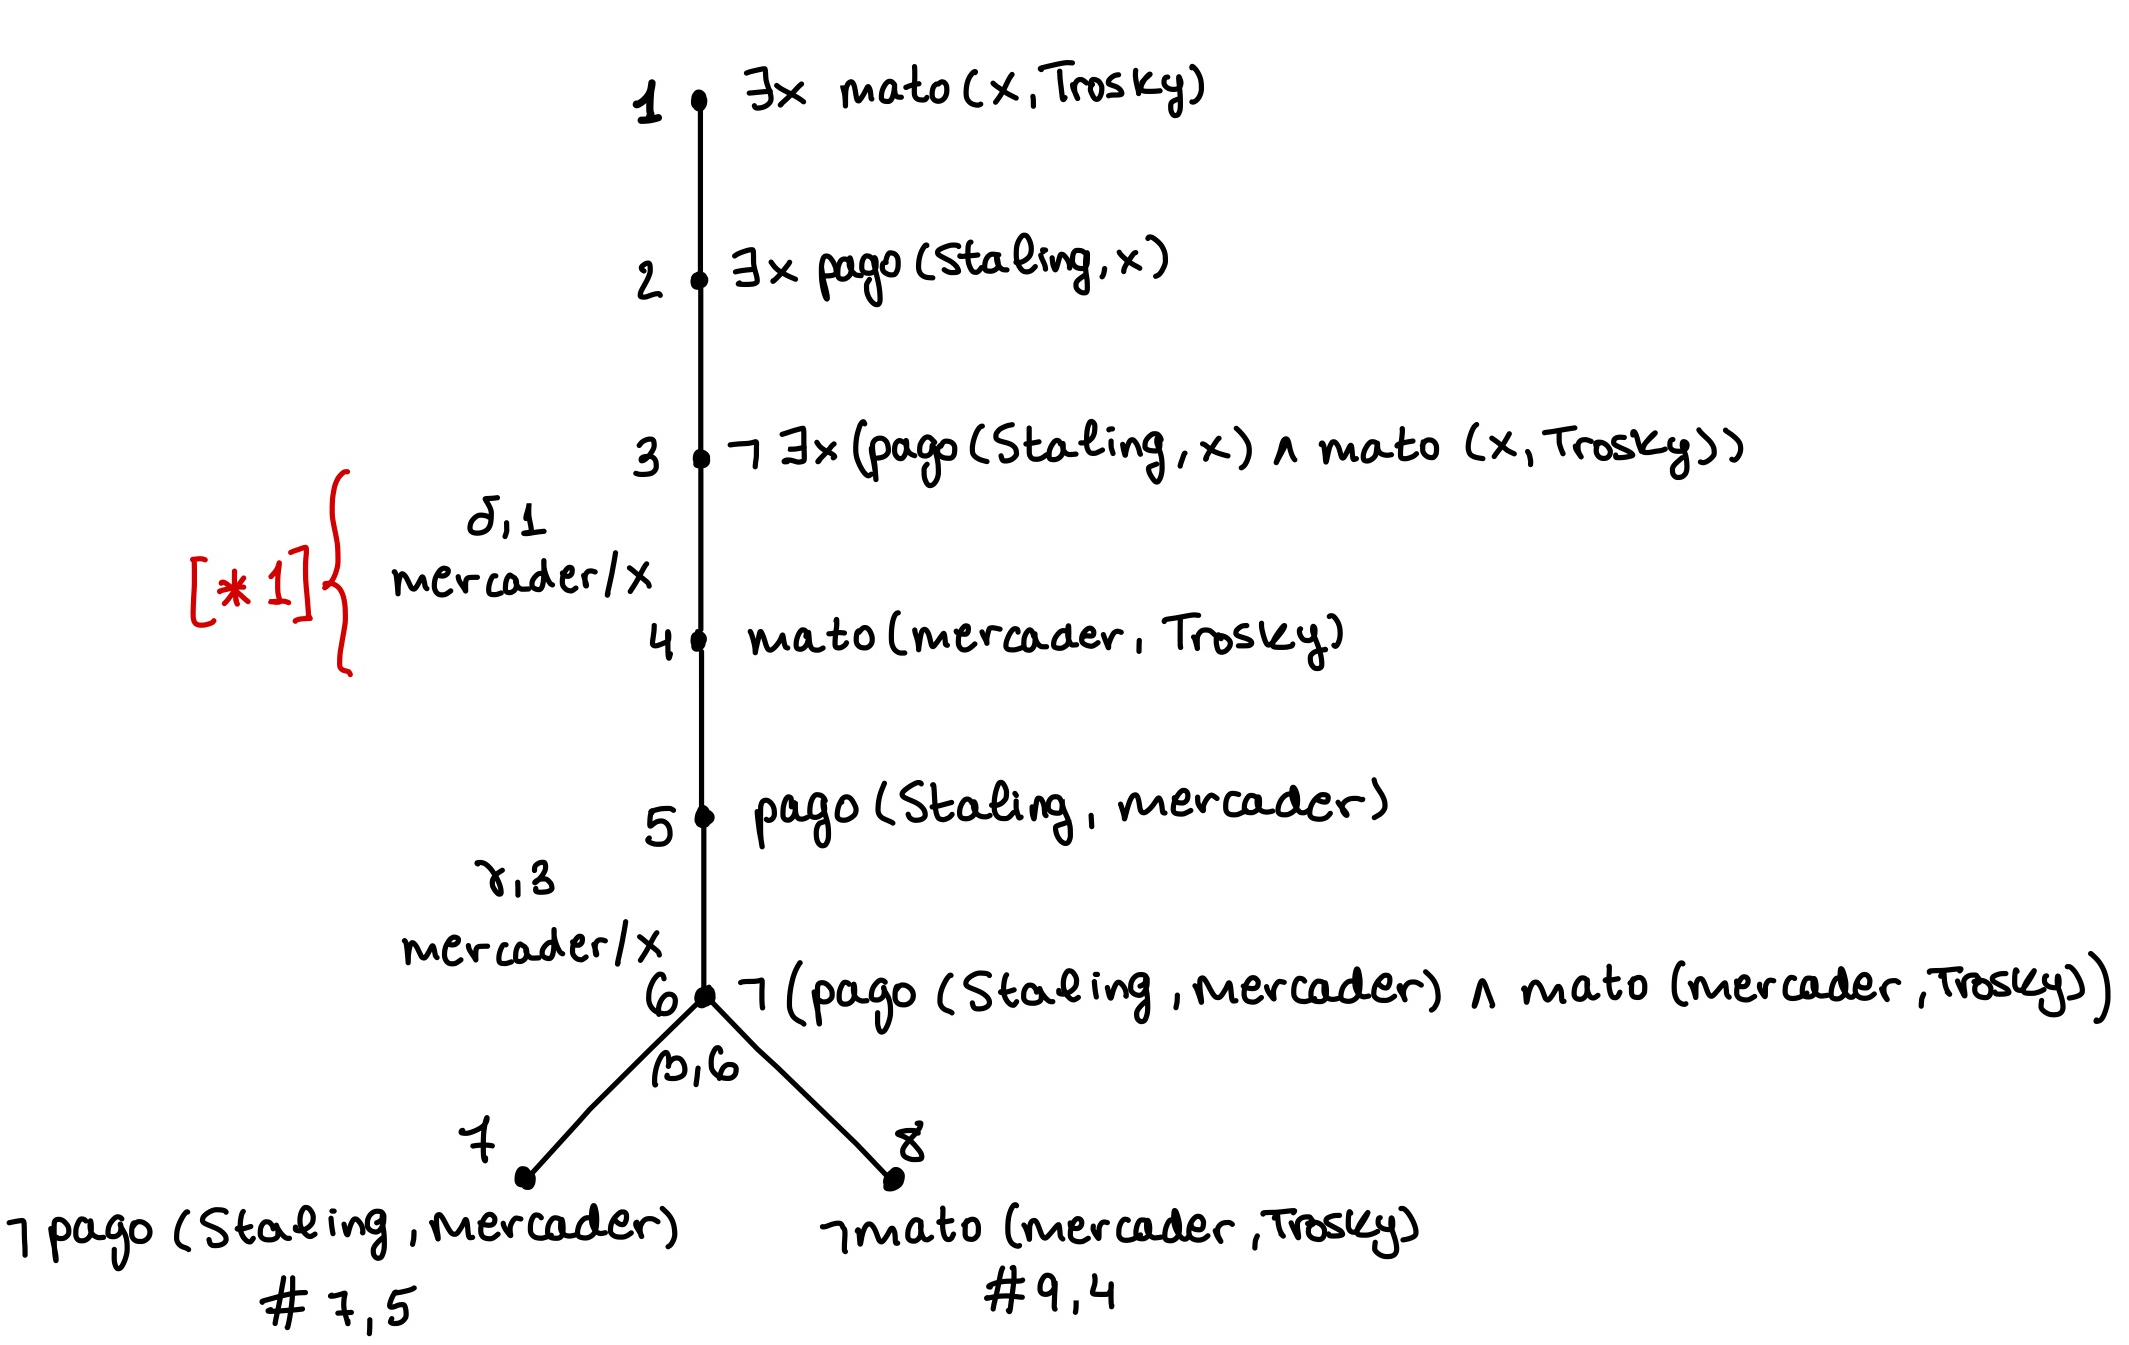
\includegraphics[width=14cm]{arbol_2.png}
\end{figure}

$[\ast 1]$ En el punto 4 hemos aplicado correctamente una regla $\delta$ introduciendo la constante auxiliar \textit{Mercader}, pero después hemos vuelto a introducirla, por tanto, estamos introduciendo una constante auxiliar que no es nueva en la rama y como consecuencia la deducción original es válida, lo que no tiene sentido.  

\begin{definition}
Dados $\Phi \subseteq \form{S}$ y $\varphi \in \form{S}$, escribimos $\tc{\Phi}{\varphi}$ cuando existe un \textbf{tableau cerrado} para $\Phi \cup \{\neg \varphi\}$.
\end{definition}

\begin{lemma}[\textbf{Correción}]
\[ \tc{\Phi}{\varphi} \Longrightarrow \Phi \models \varphi  \]
\end{lemma}

\begin{lemma}[\textbf{Completitud}]
\[ \Phi \models \varphi  \Longrightarrow \tc{\Phi}{\varphi}   \] 
\end{lemma}

\begin{lemma}
\[ \theta \in \mbox{EQ}_S, \; \models \theta  \]
\textit{Los axiomas de igualdad, son axiomas.}
\end{lemma}
\begin{proof}
\textit{Ejercicio}
\end{proof}

Para demostrar la corrección habrá que ver que las reglas de construcción de tableaux son correctas. Informalmente si una rama es satisfactible, alguna de sus extensiones lo es. 

\begin{prop}
Sean $\Phi \subseteq \form{S}$ e $\g{Y}$ una $S$-interpretación tal que $\g{Y} \models \Phi$. Entonces existe $\g{Y}'$ tal que $\g{Y} \sim_{\varphi} \g{Y}'$ para toda $\varphi \in \Phi$ y
\begin{itemize}
    \item Sea $\sigma \in \Phi$, entonces $\g{Y}' \models \Phi \cup \{\sigma_1 \}$. ($\sigma$ fórmula simplificable)
    \item Si $\alpha \in \Phi$, entonces $\g{Y}' \models \Phi \cup \{\alpha_1, \alpha_2 \}$. ($\alpha$ una $\alpha$-fórmula)
    \item Si $\beta \in \Phi$, entonces $\g{Y}' \models \Phi \cup \{\beta_1\}$ o $\g{Y}' \models \Phi \cup \{\beta_2\}$.   
    \item Si $\gamma \in \Phi$, entonces $\g{Y}' \models \Phi \cup \{\gamma(t)\}$ para $t \in TERM_S$.
    \item Si $\delta \in \Phi$, entonces $\g{Y}' \models \Phi \cup \{\delta(c)\}$ para $c \in C_A$ nueva en $\Phi$, $c \in \mbox{voc}(\Phi)$.
    \item Si $\theta \in EQ_S$, entonces $\g{Y}' \models \Phi \cup \{ \theta\}$.
\end{itemize}
\end{prop}
\begin{proof}
Los casos para $\alpha$, $\beta$ y $\sigma$ fórmulas son similares a los de la lógica proposicional. Basta usar que $\g{Y}'=\g{Y}$ y 
\[ \begin{matrix}
	\sigma \sim \sigma_1\\
	\alpha \sim \alpha_1 \wedge \alpha_2\\
	\beta \sim \beta_1 \lor \beta_2	
\end{matrix} \]
\textit{Se deja su construcción en detalle como ejercicio}. 
\paragraph{}
El caso para $\theta \in \mbox{EQ}_S$ también es trivial por el lema anterior. 
\paragraph{}
Supongamos $\gamma \in \Phi$. Supongamos $\gamma= \forall x \, \varphi$ (si $\gamma = \neg \exists \varphi$ basta usar el hecho de que es equivalente a $\forall x \neg \varphi$ y proceder como se indica). En este caso tomamos $\g{Y}'=\g{Y}$. 

Tomemos $t \in \term{S}$. Sea $a=t^{\g{Y}} \in A$. Puesto que $\forall x \varphi \in \Phi$, tenemos $\g{Y} \models \forall x \varphi$ y por tanto 
\[ \g{Y}[a/x] \models \varphi \]
Por el lema de sustitución tendremos 
\[ \g{Y} \models \varphi[t/x]  y \varphi[t/x] = \gamma(t) \]
\paragraph{}
Supongamos que $\delta \in \Phi$. Supongamos $\delta= \exists x \, \varphi$ (si $\delta = \neg \forall \varphi$ basta usar el hecho de que es equivalente a $\exists x \neg \varphi$ y proceder como se indica). Este es el único caso en el que $\g{Y}' \neq \g{Y}$.
\paragraph{}
Tomemos $c \in C_A$ nueva, $c \in \mbox{voc}(\Phi)$ ($c \not \in \mbox{voc}{\psi}, \quad \psi \in \Phi)$). $\delta(c)= \varphi[c/x]$.
\paragraph{}
Puesto que $\g{Y} \models \exists x \varphi$ y por definición existe $a \in A$ tal que $\g{Y}[a/x] \models \varphi$. 
\paragraph{}
Supongamos que $\g{Y}=\langle \g{a}, \, \sigma \rangle$. Tomemos $\g{a}'$, igual que $\g{a}$ salvo que $c^{\g{a}'}=a$. Tomemos $\g{Y}'=\langle \g{a}', \, \sigma \rangle $.
\paragraph{}
Puesto que $c \not \in \mbox{voc}(\psi)$ para $\psi \in \Phi$, tenemos que 
\[ \g{Y}' \sim_{\psi} \g{Y} \]
Por el lema de sustitución 
\[ (\varphi[c/x])^{\g{Y}'}= \varphi^{\g{Y}'[c^{\g{Y}'}/x]}=\varphi^{\g{Y}'[a/x]} \]
Al ser $c$ nueva 
\[ \g{Y}'[a/x] \sim_{\varphi} \g{Y}[a/x] \]
y de nuevo, obtenemos 
 \[ \varphi^{\g{Y}'[a/x]}= \varphi^{\g{Y}[a/x]}=\mbox{V} \]
\end{proof}